% Figure 2: Physical Parallelism vs Software Thinking
\documentclass[tikz,border=10pt]{standalone}
\usepackage{tikz}
\usetikzlibrary{shapes,arrows,positioning,calc,fit,backgrounds}

\begin{document}
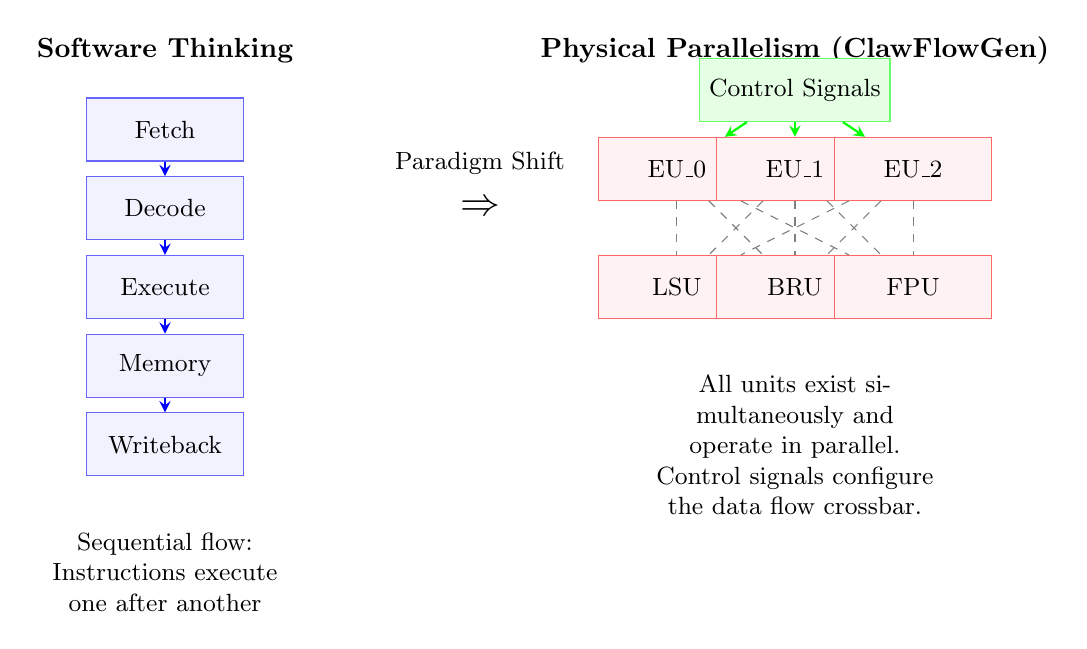
\begin{tikzpicture}[
    node distance=1.2cm,
    box/.style={rectangle, draw=black!60, fill=white, minimum width=2cm, 
                minimum height=0.8cm, text centered, font=\small},
    swbox/.style={rectangle, draw=blue!60, fill=blue!5, minimum width=2cm,
                  minimum height=0.8cm, text centered, font=\small},
    hwbox/.style={rectangle, draw=red!60, fill=red!5, minimum width=2cm,
                  minimum height=0.8cm, text centered, font=\small},
    arrow/.style={->, >=stealth},
    label/.style={font=\bfseries}
]

% Left side: Software Thinking
\node[label] at (-4, 4) {Software Thinking};

\node[swbox] (fetch) at (-4, 3) {Fetch};
\node[swbox] (decode) at (-4, 2) {Decode};
\node[swbox] (execute) at (-4, 1) {Execute};
\node[swbox] (memory) at (-4, 0) {Memory};
\node[swbox] (wb) at (-4, -1) {Writeback};

\draw[arrow, blue, thick] (fetch) -- (decode);
\draw[arrow, blue, thick] (decode) -- (execute);
\draw[arrow, blue, thick] (execute) -- (memory);
\draw[arrow, blue, thick] (memory) -- (wb);

\node[below, font=\small, text width=3cm, align=center] at (-4, -2) {
    Sequential flow:\\Instructions execute one after another
};

% Right side: Physical Parallelism
\node[label] at (4, 4) {Physical Parallelism (ClawFlowGen)};

% All operators exist simultaneously
\node[hwbox] (eu1) at (2.5, 2.5) {EU\_0};
\node[hwbox] (eu2) at (4, 2.5) {EU\_1};
\node[hwbox] (eu3) at (5.5, 2.5) {EU\_2};

\node[hwbox] (lsu) at (2.5, 1) {LSU};
\node[hwbox] (bru) at (4, 1) {BRU};
\node[hwbox] (fpu) at (5.5, 1) {FPU};

% Crossbar connections
\foreach \eu in {eu1, eu2, eu3} {
    \foreach \unit in {lsu, bru, fpu} {
        \draw[gray, thin, dashed] (\eu) -- (\unit);
    }
}

% Control signals
\node[box, fill=green!10, draw=green!60] (ctrl) at (4, 3.5) {Control Signals};
\draw[arrow, green, thick] (ctrl) -- (eu1);
\draw[arrow, green, thick] (ctrl) -- (eu2);
\draw[arrow, green, thick] (ctrl) -- (eu3);

\node[below, font=\small, text width=4cm, align=center] at (4, 0) {
    All units exist simultaneously and operate in parallel.\\
    Control signals configure the data flow crossbar.
};

% Arrow between paradigms
\node at (0, 2) {\Large$\Rightarrow$};
\node[above, font=\small] at (0, 2.3) {Paradigm Shift};

\end{tikzpicture}
\end{document}
